\documentclass{article}

\usepackage{fullpage}
\usepackage{graphicx}
\usepackage{color}
\usepackage[usestackEOL]{stackengine}
\usepackage{fancyhdr}
\usepackage{url}
\usepackage{subfig}
\usepackage{multirow}
\usepackage[table]{xcolor}
\usepackage{wrapfig}
\usepackage{amsmath,bm}
\usepackage{amssymb}
\usepackage{amsthm}
\usepackage{amsfonts}
\usepackage[round]{natbib}
\usepackage{enumitem,xcolor}
\usepackage[multiple]{footmisc}

\usepackage[
 pdftitle={Capstone Report - Udacity Machine Learning Nanodegree},
 pdfsubject={Machine Learning, Reinforcement Learning, Deep Learning, Artificial Intelligence, Games},
 pdfauthor={David Robles},
 pdfpagemode=UseOutlines,
 pdfborder= {0 0 1.0},
 bookmarks,
 bookmarksopen,
 colorlinks=true,
 citecolor=blue,
 linkcolor=blue, %
 linkbordercolor=blue, %
 urlcolor=blue, %
]{hyperref}

\usepackage{adjustbox}
\usepackage{kantlipsum}
\usepackage{tikz}
\usepackage[labelfont=bf]{caption}
\usepackage[utf8]{inputenc}

% Default fixed font does not support bold face
\DeclareFixedFont{\ttb}{T1}{txtt}{bx}{n}{8} % for bold
\DeclareFixedFont{\ttm}{T1}{txtt}{m}{n}{8}  % for normal

%%%%%%%%%%%%%
% EQUATIONS %
%%%%%%%%%%%%%

% ArgMin
\DeclareMathOperator*{\argmin}{\arg\!\min}

% ArgMax
\DeclareMathOperator*{\argmax}{\arg\!\max}

% Custom colors
\usepackage{color}
\definecolor{deepblue}{rgb}{0,0,0.5}
\definecolor{deepred}{rgb}{0.6,0,0}
\definecolor{deepgreen}{rgb}{0,0.5,0}
\definecolor{coolblue}{HTML}{101094}

\usepackage{listings}

\definecolor{codebg}{RGB}{238,238,238}

% Python style for highlighting
\newcommand\pythonstyle{\lstset{
    language=Python,
    basicstyle=\ttm,
    otherkeywords={},             % Add keywords here
    keywordstyle=\ttm\color{coolblue},
    emph={MyClass},          % Custom highlighting
    emphstyle=\ttm\color{deepred},    % Custom highlighting style
    stringstyle=\color{deepgreen},
    frame=tb,                         % Any extra options here
    framesep=10pt,
    framexleftmargin=10pt,
    backgroundcolor=\color{codebg},
    rulecolor=\color{codebg},
    aboveskip=15pt,
    belowskip=15pt,
    showstringspaces=false            % 
}}


% Python environment
\lstnewenvironment{python}[1][] {
    \pythonstyle
    \lstset{#1}
}{}

% \setmonofont[Color={0019D4}]{Courier New}


% Python for external files
\newcommand\pythonexternal[2][]{{
\pythonstyle
\lstinputlisting[#1]{#2}}}

% Python for inline
\newcommand\pythoninline[1]{{\pythonstyle\lstinline!#1!}}

%%%%%%%%%%%%%%
% Github URL %
%%%%%%%%%%%%%%

\newcommand{\GithubURL}[1]{[\href{https://github.com/davidrobles/mlnd-capstone-code/blob/master/#1}{source}]}

%%%%%%%%%%%%%%%%%%%%%%%%%%%%%%
% Connect 4 UCI Data Set URL %
%%%%%%%%%%%%%%%%%%%%%%%%%%%%%%

\newcommand{\URLUCI}{\url{https://archive.ics.uci.edu/ml/datasets/Connect-4}}

%%%%%%%%%%
% Colors % 
%%%%%%%%%%

\definecolor{even}{RGB}{205,222,231}
\definecolor{odd}{RGB}{240,249,254}
\definecolor{header}{RGB}{128,169,188}

%%%%%%%%%%%%%%%%%%%%%%%%%%%%%%%%%%%%%%%%%%%%%%%%%%%%%%%%%%%%%%%%%%%%%%%%%%%%%%%%%%%%%%%%%%%%%%%%%%%%
\title{Machine Learning Nanodegree \\ Capstone Report}
\author{David A. Robles}
\date{March 10, 2017}
\begin{document}
\maketitle
%%%%%%%%%%%%%%%%%%%%%%%%%%%%%%%%%%%%%%%%%%%%%%%%%%%%%%%%%%%%%%%%%%%%%%%%%%%%%%%%%%%%%%%%%%%%%%%%%%%%

%%%%%%%%%%%%%%%%%%%%%%%%%%%%%%%%%%%%%%%%%%%%%%%%%%%%%%%%%%%%%%%%%%%%%%%%%%%%%%%%%%%%%%%%%%%%%%%%%%%%
\section{Definition}
%%%%%%%%%%%%%%%%%%%%%%%%%%%%%%%%%%%%%%%%%%%%%%%%%%%%%%%%%%%%%%%%%%%%%%%%%%%%%%%%%%%%%%%%%%%%%%%%%%%%

%%%%%%%%%%%%%%%%%%%%%%%%%%%%%
\subsection{Project Overview}
%%%%%%%%%%%%%%%%%%%%%%%%%%%%%

Reinforcement learning is the area of machine learning concerned with the idea of learning by
interacting with an environment~\citep{Sutton1998RL}. It has a long and notable history in games.
The checkers program written by \citet{Samuel1959Checkers} was the first remarkable application of
temporal difference learning, and also the first significant learning program of any kind. It had
the principles of temporal difference learning decades before it was described and analyzed.
However, it was another game where reinforcement learning reached its first big success, when
\textsc{TD-Gammon}~\citep{Tesauro1995TD} reached world-class gameplay in Backgammon by training a
neural network-based evaluation function through self-play.

Deep Learning~\citep{LeCun2015Nature} is another branch of machine learning that allows
computational models that are composed of multiple processing layers to learn representations of
data with multiple levels of abstraction. Deep learning techniques have dramatically improved the
state-of-the-art in areas such as speech recognition~\citep{Hinton2012Speech}, image
recognition~\citep{Krizhevsky2012ImageNet} and natural language processing~\citep{Colbert2012}.

Reecently, there have been several breakthroughs when combining reinforcement learning and deep
learning. \cite{Mnih2015AtariNature} used a convolutional neural network trained with a variant of
Q-learning and learned to play Atari 2600 games at a human-level. Last year, one of the biggest
challenges for artificial intelligence was solved, when Google's DeepMind~\citep{Silver2016GoNature}
created AlphaGo to beat the world's greatest Go player. AlphaGo used deep neural networks trained by
a combination of supervised learning from human expert games, and reinforcement learning from games
of self-play.

Developing strong game-playing programs for classic two-player games (e.g. Chess, Checkers, Go) is
important in two respects: first, for humans that play the games looking for an intellectual
challenge, and second, for AI researchers that use the games as testbeds for artificial
intelligence. In both cases, the task for game programmers and AI researchers of writing strong game
AI is a hard and tedious task that requires hours of trial and error adjustments and human
expertise. Therefore, when a strong game-playing algorithm is created to play a specific game, it is
rarely useful for creating an algorithm to play another game, since the domain knowledge is
non-transferable. For this reason, there is enormous value in using machine learning to learn to
play these games without using any domain knowledge.

%%%%%%%%%%%%%%%%%%%%%%%%%%%%%%
\subsection{Problem Statement}
\label{sec:problem-statement}
%%%%%%%%%%%%%%%%%%%%%%%%%%%%%%

\newcommand{\URLcf}{https://en.wikipedia.org/wiki/Connect_Four}

In this project we use deep reinforcement learning to create an agent that learns to play the game
of \mbox{Connect 4} by playing games against itself. We define the machine learning problem as
follows:

\begin{itemize}

    \item \textbf{Task:} Playing Connect 4.

    \item \textbf{Performance:} Winning percentage when playing against other agents, and accuracy
        of the predicted outcomes on the UCI Connect 4 dataset.

    \item \textbf{Experience:} Games played against itself.

    \item \textbf{Target function:} $Q^\pi : \mathcal{S} \times \mathcal{A} \to \mathbb{R}$, where
        $\mathcal{S}$ is the set of \emph{states} (board positions) and $\mathcal{A}$ is the set of
        \emph{actions} (moves), and $\mathbb{R}$ represents the value of being in a state $s \in
        \mathcal{S}$, applying a action $a \in \mathcal{A}$, and following policy $\pi$ thereafter.

    \item \textbf{Target function representation:} Deep neural network.

\end{itemize}

More specifically, we seek to build an agent that uses Q-learning via self-play to train a deep
convolutional neural network to approximate the optimal action-value function:

\begin{equation}
Q^*(s,a) = \max\limits_\pi Q^\pi(s,a), \forall s \in \mathcal{S}, a \in \mathcal{A}
\end{equation}

\noindent which is the maximum sum of rewards achievable by a behavior policy $\pi$.

%%%%%%%%%%%%%%%%%%%%
\subsection{Metrics}
%%%%%%%%%%%%%%%%%%%%

\begin{itemize}

    \item \textbf{Winning percentage.} Consists in playing a high number of games (e.g. 100,000)
        against other agents (e.g. Alpha-Beta player) using the trained deep neural network as the
        action-value function to take greedy actions.
        
    \item \textbf{Prediction accuracy.} The learned action-value function is used to predict the
        game-theoretic outcomes (win, loss or draw) of the board positions in the Connect 4 Data
        Set.

\end{itemize}

% from wiki

% Accuracy is not a reliable metric for the real performance of a classifier, because it will yield
% misleading results if the data set is unbalanced (that is, when the number of samples in different
% classes vary greatly). For example, if there were 95 cats and only 5 dogs in the data set, the
% classifier could easily be biased into classifying all the samples as cats. The overall accuracy
% would be 95\%, but in practice the classifier would have a 100\% recognition rate for the cat class
% but a 0\% recognition rate for the dog class.

% discuss that the dataset is unbalanced

%%%%%%%%%%%%%%%%%%%%%%%%%%%%%%%%%%%%%%%%%%%%%%%%%%%%%%%%%%%%%%%%%%%%%%%%%%%%%%%%%%%%%%%%%%%%%%%%%%%%
\section{Analysis}
%%%%%%%%%%%%%%%%%%%%%%%%%%%%%%%%%%%%%%%%%%%%%%%%%%%%%%%%%%%%%%%%%%%%%%%%%%%%%%%%%%%%%%%%%%%%%%%%%%%%

%%%%%%%%%%%%%%%%%%%%%%%%%%%%%%%%%%%%%%%%%%%%%%%
\subsection{Data Exploration and Visualization}
%%%%%%%%%%%%%%%%%%%%%%%%%%%%%%%%%%%%%%%%%%%%%%%

In this project we use two environments and one dataset. The environments are the games of
Tic-Tac-Toe and Connect 4, and the dataset is the UCI Connect 4 dataset.

%%%%%%%%%%%%%%%%%%%%%%%%%%%%%%%%%%%%%%%
\subsubsection{Tic-Tac-Toe Environment}
%%%%%%%%%%%%%%%%%%%%%%%%%%%%%%%%%%%%%%%

Tic-Tac-Toe \GithubURL{capstone/game/games/tictactoe.py} is a paper-and-pencil game for two players,
X and O, who take turns marking the spaces in a 3x3 grid. The player who succeeds in placing three
of their marks in a horizontal, vertical, or diagonal row wins the game.
\hyperref[fig:tic-env]{Figure~\ref*{fig:tic-env}} shows three Tic-Tac-Toe game positions: a win, a
draw and a loss.

Tic-Tac-Toe is an extremely simple game, nonetheless, is very useful to analyze simple concepts and
to verify that the implementation of the learning algorithms are behaving as expected before moving
into the Connect 4 environment, which is more complex because of its large state space.

%%%%%%%%%%
% Figure %
%%%%%%%%%%

\begin{figure}[!b]
    \centering
    \subfloat[Win for \textsc{X}]{
        \label{fig:tic-env-win}
        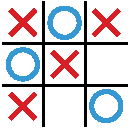
\includegraphics[width=0.15\textwidth]{figures/tic_env_win.pdf}
    } \hspace{0.2in}
    \subfloat[Win for \textsc{O}]{
        \label{fig:tic-env-loss}
        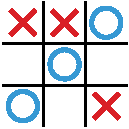
\includegraphics[width=0.15\textwidth]{figures/tic_env_loss.pdf}
    } \hspace{0.2in}
    \subfloat[Draw]{
        \label{fig:tic-env-draw}
        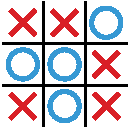
\includegraphics[width=0.15\textwidth]{figures/tic_env_draw.pdf}
    }
    \caption{Examples of a win, a loss and a draw in Tic-Tac-Toe.}
    \label{fig:tic-env}
\end{figure}

\pagebreak[4]

% \begin{python}
% from capstone.game import TicTacToe
% game = TicTacToe()
% game.legal_moves() # [1, 2, 3, 4, 5, 6, 7, 8, 9]
% print(game)
% \end{python}

%%%%%%%%%%%%%%%%%%%%%%%%%%%%%%%%%%%%%
\subsubsection{Connect 4 Environment}
%%%%%%%%%%%%%%%%%%%%%%%%%%%%%%%%%%%%%

Connect 4 \GithubURL{capstone/game/games/connect4.py} is a two-player board game of perfect
information where pieces are dropped into the columns of a vertical $6 \times 7$ grid with the goal
of forming a straight line of 4 connected pieces. There are at most seven actions per state, since
placing a piece in a column is a legal action only if that column has at least one empty location.
In this project we use pieces of two colors: \textsc{Yellow} for the first player, and \textsc{Red}
for the second player. \hyperref[fig:c4-env]{Figure~\ref*{fig:c4-env}} shows three Connect 4 game
positions: a win, a draw and a loss:

%%%%%%%%%%
% Figure %
%%%%%%%%%%

\begin{figure}[!h]
    \centering
    \subfloat[Win for \textsc{Yellow}]{
        \label{fig:c4-env-wing}
        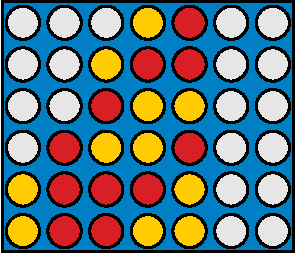
\includegraphics[width=0.18\textwidth]{figures/c4_env_win.pdf}
    } \hspace{0.1in}
    \subfloat[Win for \textsc{Red}]{
        \label{fig:c4-env-loss}
        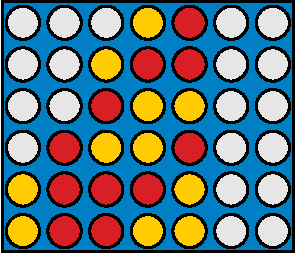
\includegraphics[width=0.18\textwidth]{figures/c4_env_loss.pdf}
    } \hspace{0.1in}
    \subfloat[Draw]{
        \label{fig:c4-env-draw}
        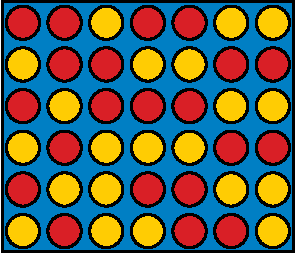
\includegraphics[width=0.18\textwidth]{figures/c4_env_draw.pdf}
    }
    \caption{Examples of a win, a loss and a draw in Connect Four.}
    \label{fig:c4-env}
\end{figure}


%%%%%%%%%%%%%%%%%%%%%%%%%%%%%%%%%%%%%%
\subsubsection{UCI Connect 4 Data Set}
%%%%%%%%%%%%%%%%%%%%%%%%%%%%%%%%%%%%%%

As part of the testing phase, we will use the \emph{Connect 4 Data Set}\footnote{\URLUCI{}} that is
available from the UCI Machine Learning Repository~\citep{Hettich1998UCI}. A partial view of the
dataset is presented in \hyperref[table:uci-dataset]{Table~\ref*{table:uci-dataset}}. The dataset
has a total of 67,557 instances, representing all legal 8-ply positions in \mbox{Connect 4} in which
neither player has won yet, and which the next move is not forced. Each instance is described by 42
features, one for each space in the $6 \times 7$ board, and can belong to one of the classes
$\{\texttt{x}, \texttt{o}, \texttt{b}\}$, where \texttt{x} is the first player, \texttt{o} is the
second player, and \texttt{b} is empty. The outcome class is the game theoretical value for the
first player, and can belong to one of the classes $\{\texttt{win}, \texttt{loss}, \texttt{draw}\}$.
There are 44,473 wins, 16,635 losses and 6,449 draws \GithubURL{examples/c4_uci_data_expl.py}.
\hyperref[fig:c4-exp]{Figure~\ref*{fig:c4-exp}} shows a visual representation of five randomly
selected instances of the data set. As we can see, all game positions have eight pieces in the
board, representing all legal 8-ply positions \GithubURL{examples/c4_uci_viz.py}.

%%%%%%%%%%%%%%%%%%%%%%
% Table: UCI Dataset %
%%%%%%%%%%%%%%%%%%%%%%

\begin{table}[b!]
\small
\centering
\renewcommand{\arraystretch}{1.2}
{\rowcolors{3}{even}{odd}
\begin{tabular}{ c | c c c c c c c c c c c c c c c c c | c }
\rowcolor{header}
 & \multicolumn{17}{c|}{\textbf{Features}} &  \textbf{Target} \\ \rowcolor{header}
\textbf{No.} & \textbf{a1} & \textbf{a2} & \textbf{a3} & \textbf{a4} & \textbf{a5} &
    \textbf{a6} & \textbf{b1} & \textbf{b2} & \textbf{...} & \textbf{f5} & \textbf{f6} &
    \textbf{g1} & \textbf{g2} & \textbf{g3} & \textbf{g4} & \textbf{g5} & \textbf{g6} & \textbf{outcome} \\ 
0      &  b &  b &  b &  b &  b &  b &  b &  b & ... &  b &  b &  b &  b &  b &  b &  b &  b &     win \\
1      &  b &  b &  b &  b &  b &  b &  b &  b & ... &  b &  b &  b &  b &  b &  b &  b &  b &     win \\
2      &  b &  b &  b &  b &  b &  b &  o &  b & ... &  b &  b &  b &  b &  b &  b &  b &  b &     win \\
3      &  b &  b &  b &  b &  b &  b &  b &  b & ... &  b &  b &  b &  b &  b &  b &  b &  b &     win \\
4      &  o &  b &  b &  b &  b &  b &  b &  b & ... &  b &  b &  b &  b &  b &  b &  b &  b &     win \\
...    & .. & .. & .. & .. & .. & .. & .. & .. & ... & .. & .. & .. & .. & .. & .. & .. & .. &     ... \\
67552  &  x &  x &  b &  b &  b &  b &  o &  x & ... &  b &  b &  o &  o &  x &  b &  b &  b &    loss \\
67553  &  x &  x &  b &  b &  b &  b &  o &  b & ... &  b &  b &  o &  x &  o &  o &  x &  b &    draw \\
67554  &  x &  x &  b &  b &  b &  b &  o &  o & ... &  b &  b &  o &  x &  x &  o &  b &  b &    loss \\
67555  &  x &  o &  b &  b &  b &  b &  o &  b & ... &  b &  b &  o &  x &  o &  x &  x &  b &    draw \\
67556  &  x &  o &  o &  o &  x &  b &  o &  b & ... &  b &  b &  x &  b &  b &  b &  b &  b &    draw \\
\end{tabular}
}
\caption{UCI Connect 4 Dataset. Each row represents a different board position, and each feature
         represents a specific cell in the board. The target is the outcome of the game for the
         first player, assuming perfect play.}
\label{table:uci-dataset}
\end{table}

\pagebreak[4]

%%%%%%%%%%
% Figure %
%%%%%%%%%%

\begin{figure}[!t]
    \centering
    \subfloat[Win]{
        \label{fig:c4-exp-1}
        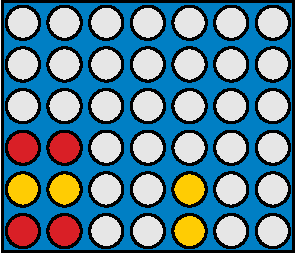
\includegraphics[width=0.15\textwidth]{figures/c4_exploration_1_win.pdf}
    } \hspace{0.1in}
    \subfloat[Loss]{
        \label{fig:c4-exp-2}
        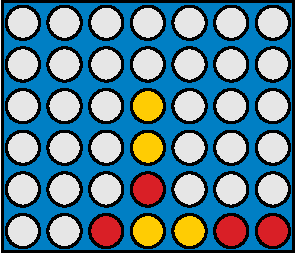
\includegraphics[width=0.15\textwidth]{figures/c4_exploration_2_loss.pdf}
    } \hspace{0.1in}
    \subfloat[Win]{
        \label{fig:c4-exp-3}
        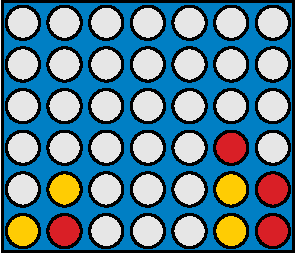
\includegraphics[width=0.15\textwidth]{figures/c4_exploration_3_win.pdf}
    } \hspace{0.1in}
    \subfloat[Loss]{
        \label{fig:c4-exp-4}
        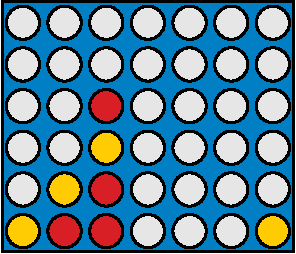
\includegraphics[width=0.15\textwidth]{figures/c4_exploration_4_loss.pdf}
    } \hspace{0.1in}
    \subfloat[Draw]{
        \label{fig:c4-exp-10}
        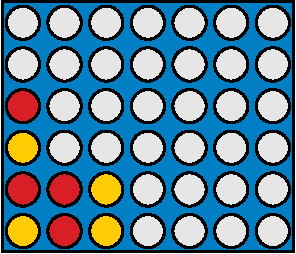
\includegraphics[width=0.15\textwidth]{figures/c4_exploration_10_draw.pdf}
    }
    \caption{Five randomly selected instances of the UCI Connect 4 Data Set. The outcome of each board
    position is from the point of view of the firs player (Yellow discs).}
    \label{fig:c4-exp}
\end{figure}

%%%%%%%%%%%%%%%%%%%%%%%%%%%%%%%%%%%%%%
\subsection{Algorithms and Techniques}
%%%%%%%%%%%%%%%%%%%%%%%%%%%%%%%%%%%%%%

%%%%%%%%%%%%%%%%%%%%%%%%%%%%%%%%%%%%%%%
\subsubsection{Markov Decision Process}
%%%%%%%%%%%%%%%%%%%%%%%%%%%%%%%%%%%%%%%

A \emph{Markov decision process} (MDP) consist of four elements:

\begin{itemize}

    \item $\mathcal{S}$ is the set of \emph{states} (state space).

    \item $\mathcal{A}$ is the set of \emph{actions} (action space). The set of actions that are
        available in some particular state $s_t \in \mathcal{S}$ is denoted $\mathcal{A}(s_t)$.

    \item $ T : \mathcal{S} \times \mathcal{A} \times \mathcal{S} \to \mathbb{R}$ is the
      \emph{transition function}, which is the probability given we are in state $s_t \in
      \mathcal{S}$, take action $a_t \in \mathcal{A}(s_t)$ and we will transition to state $s_{t+1}
      \in \mathcal{S}$.

    \item $ R : \mathcal{S} \times \mathcal{A} \times \mathcal{S} \to \mathbb{R}$ is the
      \emph{reward function}, which is the immediate reward received when in state $s_t \in
      \mathcal{S}$ action $a_t \in \mathcal{A}$ is taken and the MDP transitions to state $s_{t+1}
      \in \mathcal{S}$. However, it is also possible to define it either as $ R : \mathcal{S} \times
      \mathcal{A} \to \mathbb{R}$ or $R : \mathcal{S} \to \mathbb{R}$. The first one gives rewards
      for performing an action $a_t$ in a particular state $s_t$, and the second gives rewards when
      transitioning to state $s_{t+1}$.

\end{itemize}

%%%%%%%%%%%%%%%%%%%%%%%%%%%
\subsubsection{Environment}
%%%%%%%%%%%%%%%%%%%%%%%%%%%

In the reinforcement learning problem an agent does not have access to the dynamics (reward and
transition function) of the MDP. However, it interacts with an \emph{environment} by way of three
signals: a \emph{state}, which describes the state of the environment, an \emph{action}, which
allows the agent to have some impact on the environment, and a \emph{reward}, which provides the
agent with feedback on its immediate performance.

%%%%%%%%%%%%%%%%%%%%%%
\subsubsection{Policy}
%%%%%%%%%%%%%%%%%%%%%%

% \GithubURL{capstone/policy/policy.py}{Implementation}

In an MDP, the agent acts according to a policy $\pi$, which maps each state $s \in \mathcal{S}$ to
an action $a \in \mathcal{A}(s)$. A policy that specifies a unique action to be performed is called
a \emph{deterministic} policy, and is defined as $\pi : \mathcal{S} \rightarrow \mathcal{A}$.

The interaction between the policy used by the agent and the environment works as follows. First, it
starts at an \emph{initial state} $s_0$. Then, the policy $\pi$ selects an action $a_0 = \pi(s_0)$
from the set of available actions $\mathcal{A}(s_0)$, and the action is executed. The environment
transitions to a new state $s_1$ based on the transition function $T$ with probability
$T(s_0,a_0,s_1)$, and a reward $r_0 = R(s_0, a_0, s_1)$ is received. This process continues,
producing a \emph{trajectory} of experience $s_0, a_0, s_1, r_1, a_1, s_2, r_2, a_2, \dots$, and the
process ends in a \emph{terminal state} $s_T$ and is restarted in the initial state.

We use three types of policies in this project:

\begin{itemize}

    \item \textbf{Random.} Selects actions uniformly at random.

    \item \textbf{Greedy.} Selects the \emph{max action}, which is the greedy
                           action with the highest value,

        \begin{equation}
            \pi_{\textrm{greedy}}(s) = \argmax_{a \in \mathcal{A}(s)} Q(s, a)
        \end{equation}

    \item \textbf{$\epsilon$-greedy.} Selects the best action for a proportion
        $1 - \epsilon$ of the trials, and another action is randomly selected (with
        uniform probability) for a proportion,

        \begin{equation}
            \pi_{\epsilon}(s) = \left\{
             \begin{array}{lr}
                 \pi_{\textrm{rand}}(s,a) & \text{if } rand() < \epsilon\\
                 \pi_{\textrm{greedy}}(s,a) & \text{otherwise}
             \end{array}
           \right.
        \end{equation}

        where $\epsilon \in [0, 1]$ and $rand()$ returns a random number from a
        uniform distribution $\in [0, 1]$.

\end{itemize}

%%%%%%%%%%%%%%%%%%%%%%%%%%%%%%%
\subsubsection{Value Functions}
%%%%%%%%%%%%%%%%%%%%%%%%%%%%%%%

Most of the algorithms for solving MDPs (computing optimal policies) do it by learning a \emph{value
function}. A value function estimates what is good for an agent over the long run. It estimates the
expected outcome from any given state, by summarising the total amount of reward that an agent can
expect to accumulate into a single number. Value functions are defined for particular policies.

Two types of value functions exist: state value functions and action value functions. In this
project, however, we only focus in the latter.

The \emph{action value function} (or Q-function), is the expected return after selecting action $a$
in state $s$ and then following policy $\pi$,
%
\begin{equation}
Q^\pi(s,a) = \mathbb{E}_\pi \left[ R_t | s_t = s, a_t = a \right]
\end{equation}

The \emph{optimal value function} is the unique value function that maximises the value of every
state, or state-action pair,
%
\begin{eqnarray}
Q^*(s,a) & = & \max\limits_\pi Q^\pi(s,a), \forall s \in \mathcal{S}, a \in \mathcal{A}
\end{eqnarray}

An \emph{optimal policy} $\pi^*(s,a)$ is a policy that maximises the action value function from
every state in the MDP,
%
\begin{equation}
    \pi^*(s,a) = \argmax_\pi Q^\pi(s, a)
\end{equation}

%%%%%%%%%%%%%%%%%%%%%%%%%%
\subsubsection{Q-learning}
%%%%%%%%%%%%%%%%%%%%%%%%%%

One of the most basic and popular methods to estimate action-value functions is the
\emph{Q-learning} algorithm~\citep{Watkins1989PhD} \GithubURL{capstone/rl/learners/qlearning.py}.
It is model-free online off-policy algorithm, whose main strength is that it is able to compare the
expected utility of the available actions without requiring a model of the environment. Q-learning
works by learning an action-value function that gives the expected utility of taking a given action
in a given state and following a fixed policy thereafter. The update rule uses action-values and a
built-in max-operator over the action-values of the next state in order to update $Q(s_t, a_t)$ as
follows,
%
\begin{equation} Q(s_t, a_t) \gets Q(s_t, a_t) + \alpha [r_{t+1} + \gamma \max_a Q(s_{t+1}, a) -
Q(s_t, a_t)] \end{equation}

The agent makes a step in the environment from state $s_t$ to $s_{t+1}$ using action $a_t$ while
receiving reward $r_t$. The update takes place on the action-value $a_t$ in the state $s_t$ from
which this action was executed. This version of Q-learning works well for tasks with a small a
state-space, since it uses arrays or tables with one entry for each state-action pair. In many cases
in which there are far more states than could possibly be entries in a table we need to use function
approximation.

%%%%%%%%%%%%%%%%%%%%%%%%%%%%%%%%%%%%%%
\subsubsection{Approximate Q-learning}
%%%%%%%%%%%%%%%%%%%%%%%%%%%%%%%%%%%%%%

Function approximation consists in using a more compact parameterized function representations,
instead of the tabular case.

It is possible to use a function approximator to estimate the action-value function, $Q(s,a;\theta)
\approx Q(s,a)$.

% We refer to a neural network function approximator with weights $\theta$ as a Q-network.

% asfd asd fas fd asf as fsaasfd asd fas fd asf as fsaasfd asd fas fd asf as fsaasfd asd fas fd asf as
% fsaasfd asd fas fd asf as fsaasfd asd fas fd asf as fsaasfd asd fas fd asf as fsaasfd asd fas fd asf
% as fsaasfd asd fas fd asf as fsaasfd asd fas fd asf as fsaasfd asd fas fd asf as fsaasfd asd fas fd
% asf as fsaasfd asd fas fd asf as fsaasfd asd fas fd asf as fsaasfd asd fas fd asf as fsa

% \GithubURL{capstone/rl/learners/qlearning.py}.

%%%%%%%%%%%%%%%%%%%%%%%%%
\subsubsection{Self-play}
%%%%%%%%%%%%%%%%%%%%%%%%%

% \GithubURL{capstone/rl/learners/qlearning_selfplay.py}{Implementation}

Self-play is by far the most popular training method. It is a single policy $\pi(s,a)$ that is used
by both players in a two-player game, $\pi_1(s,a) = \pi_2(s,a) = \pi(s,a)$. The first reason for its
popularity is that training is quickest if the learner's opponent is roughly equally strong, and
that definitely holds for self-play. As a second reason for popularity, there is no need to
implement or access a different agent with roughly equal playing strength. However, self-play has
several drawbacks, with the main one being that a single opponent does not provide sufficient
exploration~\citep{Szita2011RLGames}.

%%%%%%%%%%%%%%%%%%%%%%%%%%%%%%%%%%
\subsubsection{Alpha-beta pruning}
%%%%%%%%%%%%%%%%%%%%%%%%%%%%%%%%%%

\emph{Alpha-beta pruning}~\citep{Knuth1975AB} \GithubURL{capstone/game/players/alphabeta.py} is the
most common game tree search algorithm for two-player games of perfect information. It extends the
minimax algorithm to reduce the number of nodes that are evaluated in the game tree. Instead of
calculating the exact minimax values for all the nodes in the game tree, alpha-beta prunes away
branches that will not have any effect in the selection of the best move.

%%%%%%%%%%%%%%%%%%%%%%
\subsection{Benchmark}
\label{sec:benchmark}
%%%%%%%%%%%%%%%%%%%%%%

\begin{itemize}

    \item \textbf{Random agent}. This benchmark consists in playing against an agent that takes
        uniformly random moves. This is the most basic benchmark, but first we have to be sure that
        our learned evaluation function can play better than a random agent before moving into a
        harder benchmark. Also, this will help us to detect bugs in the code and algorithms: if a
        learned value function does not play significantly better than a random agent, is not
        learning. The idea is to test against this benchmark using Alpha-beta pruning at 1, 2 and
        4-ply search.

    \item \textbf{Connect 4 Data Set}. This dataset will be used as the main benchmark. The learned
        value function will be used to predict the game-theoretic outcomes (win, loss or draw) for
        the first player in the 67,557 instances of the dataset.

\end{itemize}


%%%%%%%%%%%%%%%%%%%%%%%%%%%%%%%%%%%%%%%%%%%%%%%%%%%%%%%%%%%%%%%%%%%%%%%%%%%%%%%%%%%%%%%%%%%%%%%%%%%%
\section{Methodology}
%%%%%%%%%%%%%%%%%%%%%%%%%%%%%%%%%%%%%%%%%%%%%%%%%%%%%%%%%%%%%%%%%%%%%%%%%%%%%%%%%%%%%%%%%%%%%%%%%%%%

%%%%%%%%%%%%%%%%%%%%%%%%%%%%%%%%%%%%%%%%%%%%%%%%%%%%%%%%%%%%%%%%%%%%%%%%%%
\subsection{Data Preprocessing}
%%%%%%%%%%%%%%%%%%%%%%%%%%%%%%%%%%%%%%%%%%%%%%%%%%%%%%%%%%%%%%%%%%%%%%%%%%

Content.

\pagebreak[4]

%%%%%%%%%%%%%%%%%%%%%%%%%%%%%%%%%%%%%%%%%%%%%%%%%%%%%%%%%%%%%%%%%%%%%%%%%%
\subsection{Implementation}
%%%%%%%%%%%%%%%%%%%%%%%%%%%%%%%%%%%%%%%%%%%%%%%%%%%%%%%%%%%%%%%%%%%%%%%%%%

%%%%%%%%%%%%%%%%%%%%%%%%%%%%%%%%%%%%%%%
\subsubsection{Game}
%%%%%%%%%%%%%%%%%%%%%%%%%%%%%%%%%%%%%%%

The first part of the implementation was to implement the two games, Tic-Tac-Toe and Connect 4. The
idea was to design them first in a way that is independent of reinforcement learning. The following
is the abstract Game interface for both \GithubURL{capstone/game/game.py}.

\begin{python}
class Game(object):

    def copy(self):
        '''Returns a copy of the game.'''
        pass

    def cur_player(self):
        '''
        Returns the index of the player in turn, starting with 0:
        0 (Player 1), 1 (Player 2), etc.
        '''
        pass

    def is_over(self):
        '''Returns True if the game is over.'''
        return len(self.legal_moves()) == 0

    def legal_moves(self):
        '''Returns a list of legal moves for the player in turn.'''
        pass

    def make_move(self, move):
        '''Makes one move for the player in turn.'''
        pass

    def make_moves(self, moves):
        '''Makes a series of moves.'''
        pass

    def outcomes(self):
        '''Returns a list of outcomes for each player at the end of the game.'''
        pass

    def outcome(self, player_idx):
        '''Returns the outcome for the given player.'''
        pass

    def reset(self):
        '''Restarts the game.'''
        pass
\end{python}

Once we had the Game interface well defined we implemented both Tic-Tac-toe
\GithubURL{capstone/game/games/tictactoe.py} and \mbox{Connect 4}
\GithubURL{capstone/game/games/tictactoe.py}.

%%%%%%%%%%%%%%%%%%%%%%%%%%%%%%%%%%%%%%%
\subsubsection{Markov Decision Process}
%%%%%%%%%%%%%%%%%%%%%%%%%%%%%%%%%%%%%%%

We then designed the interface for an MDP \GithubURL{capstone/rl/mdp.py} as follows:

\begin{python}
class MDP(object):

    def states(self):
        '''Returns a list of all states. Not generally possible for large MDPs.'''
        pass

    def start_state(self):
        '''Returns the initial state.'''
        pass

    def actions(self, state):
        '''Returns a list of possible actions in the given state.'''
        pass

    def transitions(self, state, action):
        '''
        Returns a dict of (next_state: probability) key/values, where 'next_state' is
        reachable from 'state' by taking 'action'. The sum of all probabilities should
        be 1.0. Not available in reinforcement learning.
        '''
        pass

    def reward(self, state, action, next_state):
        '''
        Returns the reward of being in 'state', taking 'action', and ending up
        in 'next_state'. Not available in reinforcement learning.
        '''
        pass

    def is_terminal(self, state):
        '''.Returns True if the given state is terminal.'''
        pass
\end{python}

%%%%%%%%%%%%%%%%%%%%%%%%%%%%%%%%%%%%%%%%%%%%%
\subsubsection{Converting a Game into an MDP}
%%%%%%%%%%%%%%%%%%%%%%%%%%%%%%%%%%%%%%%%%%%%%

Content.

\pagebreak[4]

%%%%%%%%%%%%%%%%%%%%%%%%%%%
\subsubsection{Environment}
%%%%%%%%%%%%%%%%%%%%%%%%%%%

A reinforcement learning environment \GithubURL{capstone/rl/environment.py} for interacting with an
MDP. The main idea is that it restricts access to the transition and reward functions. It needs to
interact with the environment to transition to another state and receive rewards.

\begin{python}
class Environment(object):

    def __init__(self, mdp):
        self._mdp = mdp
        self._cur_state = self._mdp.start_state()

    def actions(self, state):
        '''Returns the available actions in the given state.'''
        return self._mdp.actions(state)

    def cur_state(self):
        '''Returns the current state.'''
        return self._cur_state.copy()

    def do_action(self, action):
        '''
        Performs the given action in the current state.
        Returns (reward, next_state).
        '''
        prev = self.cur_state()
        transitions = self._mdp.transitions(self.cur_state(), action)
        for next_state, prob in transitions:
            self._cur_state = next_state
        reward = self._mdp.reward(prev, action, self.cur_state())
        return reward, self.cur_state()

    def is_terminal(self):
        return self._mdp.is_terminal(self.cur_state())

    def reset(self):
        '''Resets the current state to the start state.'''
        self._cur_state = self._mdp.start_state()
\end{python}

%%%%%%%%%%%%%%%%%%%%%%%
\subsubsection{Learner}
%%%%%%%%%%%%%%%%%%%%%%%

We define an episodic learner. It is basically an interface for algorithms that learn a value
function by interacting with an environment in an episodic way.

\begin{python}
class Learner(object):

    def __init__(self, env, n_episodes=1000):
        self.env = env
        self.n_episodes = n_episodes

    def train(self, callbacks=None):
        '''Trains the model for a fixed number of episodes.'''
        callbacks = CallbackList(callbacks)
        callbacks.on_train_begin()
        for episode in range(self.n_episodes):
            callbacks.on_episode_begin(episode)
            self.env.reset()
            self.episode()
            callbacks.on_episode_end(episode, self.qfunction)
        callbacks.on_train_end(self.qfunction)

    @abc.abstractmethod
    def episode(self):
        pass
\end{python}

\pagebreak[4]

%%%%%%%%%%%%%%%%%%%%%%%%%%%%%%%%%%
\subsubsection{Tabular Q-learning}
%%%%%%%%%%%%%%%%%%%%%%%%%%%%%%%%%%

asdf asd fas fas df a.

\begin{python}
class QLearning(Learner):
    '''Tabular Q-learning'''

    def __init__(self, env, policy, qfunction, learning_rate=0.1, discount_factor=1.0):
        super(QLearning, self).__init__(env, **kwargs)
        self.policy = policy
        self.qfunction = qfunction
        self.learning_rate = learning_rate
        self.discount_factor = discount_factor

    def best_qvalue(self, state):
        return max_qvalue(state, self.env.actions(state), self.qfunction)

    def episode(self):
        while not self.env.is_terminal():
            state = self.env.cur_state()
            action = self.policy.action(state)
            reward, next_state = self.env.do_action(action)
            best_qvalue = self.best_qvalue(next_state)
            target = reward + (self.discount_factor * best_qvalue)
            td_error = target - self.qfunction[state, action]
            self.qfunction[state, action] += self.learning_rate * td_error
\end{python}

%%%%%%%%%%%%%%%%%%%%%%%%%%%%%%%%%%%%%%
\subsubsection{Approximate Q-learning}
%%%%%%%%%%%%%%%%%%%%%%%%%%%%%%%%%%%%%%

\begin{python}
class ApproximateQLearning(Learner):
    '''Q-learning with a function approximator'''

    def __init__(self, env, policy, qfunction, discount_factor=1.0,
                 experience_replay=True, **kwargs):
        super(ApproximateQLearning, self).__init__(env, **kwargs)
        self.policy = policy
        self.qfunction = qfunction
        self.discount_factor = discount_factor
        self.experience_replay = experience_replay
        if self.experience_replay:
            self.memory = set()

    def best_qvalue(self, state):
        return max_qvalue(state, self.env.actions(state), self.qfunction)

    def episode(self):
        while not self.env.is_terminal():
            state = self.env.cur_state()
            action = self.policy.action(state)
            reward, next_state = self.env.do_action(action)
            if self.experience_replay:
                self.memory.add((state, action, reward, next_state))
                state, _, reward, next_state = random.choice(tuple(self.memory))
            best_qvalue = self.best_qvalue(next_state)
            update = reward + (self.discount_factor * best_qvalue)
            self.qfunction.update(state, update)

\end{python}

%%%%%%%%%%%%%%%%%%%%%%%%%%%%%%%%%%%%%%%%%%%%%%%%%%%%%%%%%%%%%%%%%%%%%%%%%%
\subsection{Refinement}
%%%%%%%%%%%%%%%%%%%%%%%%%%%%%%%%%%%%%%%%%%%%%%%%%%%%%%%%%%%%%%%%%%%%%%%%%%

Content.

%%%%%%%%%%%%%%%%%%
\subsection{Games}
%%%%%%%%%%%%%%%%%%

%%%%%%%%%%%%%%%%%%%%%%%%%%%
\subsubsection{Tic Tac Toe}
%%%%%%%%%%%%%%%%%%%%%%%%%%%

% \GithubURL{capstone/game/tictactoe.py}{Implementation}

\subsubsection{GameMDP converter}

Converting an MDP

%%%%%%%%%%%%%%%%%%%%%%%%%%%%%%%%%%%%%%%%%%%%%%%%%%%%%%%%%%%%%%%%%%%%
\section{Examples}
%%%%%%%%%%%%%%%%%%%%%%%%%%%%%%%%%%%%%%%%%%%%%%%%%%%%%%%%%%%%%%%%%%%%

%%%%%%%%%%%%%%%%%%%%%%%%%%%%%%%%%%%%%%%%%%%%%%%%%%%%%%%%%%%%%%%%%%
\subsection{Estimate state-action values using tabular Q-learning}
%%%%%%%%%%%%%%%%%%%%%%%%%%%%%%%%%%%%%%%%%%%%%%%%%%%%%%%%%%%%%%%%%%

In this example we will estimate the state-action values for two very simple board positions for
both Tic-Tac-Toe and Connect 4. We will be using the tabular version of Q-learning. The goal here is
simply to verify that our implementation of the Q-learning algorithm is working as expected. We
chose very simple positions because the expected q-values are easy to understand.

We converted both games as MDPs by making the opponent a fixed agent that takes optimal moves by
using the Alpha-Beta algorithm. This allowed us to verify that we are learning the q-values assuming
the worst case scenario. In other situations in which the depth of the game tree is huge Alpha-Beta
would need to combined with a good heuristic evaluation function, but in these simple positions it
won't be necessary.

The rewards given by the Tic-Tac-Toe environment are $+1$ for a win for the first player, $-1$ for a
win for the first player, and $0$ for a draw.

%%%%%%%%%%%%%%%%%%%%%%%%%%%
\subsubsection{Tic-Tac-toe}
%%%%%%%%%%%%%%%%%%%%%%%%%%%

% - Implement Q-learning
% - GameMDP converter
% - Generate a Tic-Tac-Toe board that is easier to analyze
% - Run Q-learning and show that the values are correct.

% \GithubURL{examples/tic_ql_tab_full.py}{Implementation}

For Tic-Tac-Toe we used the board position in \hyperref[fig:tic-ql-tab-cur]
{Figure~\ref*{fig:tic-ql-tab-cur}} as the starting state, $s_0$. It has five available actions,
$\mathcal{A}(s_0) = \{1, 2, 4, 6, 9\}$. By looking at such a simple position we can clearly identify
that the best available action is 9, which leads to a win if we keep playing the best possible
actions. Any other action (i.e. 1, 2, 4 or 6) would lead to a loss, assuming perfect play from the
opponent.

\begin{figure}[!h]
    \centering
    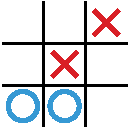
\includegraphics[width=0.15\textwidth]{figures/tic_ql_tab_current.pdf}
    \caption{Starting Tic-Tac-Toe state, $s_0$, with five legal actions, $\mathcal{A}(s_0) = \{1, 2, 4, 6, 9\}$.}
    \label{fig:tic-ql-tab-cur}
\end{figure}

We ran the tabular version of the Q-learning algorithm with $\alpha = 0.1$ (learning rate),
$\gamma=1.0$ (discount factor), and a uniformly random behavior policy. The Q-values converged to
the expected values after around 800 episodes of training, and are shown in
\hyperref[fig:tic-ql-qvalues] {Figure~\ref*{fig:tic-ql-qvalues}}. As we can see in
\hyperref[fig:tic-ql-tab-move-9] {Figure~\ref*{fig:tic-ql-tab-move-9}}, the expected future reward
of taking action 9 is correctly estimated as 1.0, since that would lead to a win. At the same time,
the q-values for all the other actions was -1.0. This makes sense, since any action not being 9
would lead to an immediate loss. Also, we can see in \hyperref[fig:tic-ql-tab-qvalues-progress]
{Figure~\ref*{fig:tic-ql-tab-qvalues-progress}} we can see the predicted q-values for each available
action. It is interesting to see how the q-value for $Q(s_0, 9)$ takes some time to converge. This
is probably because taking action 9 leads to an eventual win, but not immediately. It requires
making another move (either 1 or 6) to win.

% show the index numbers of the board

%%%%%%%%%%
% Figure %
%%%%%%%%%%

\begin{figure}[!h]
    \centering
    \subfloat[$Q(s_0, 1) = -1.0$]{
        \label{fig:tic-ql-tab-move-1}
        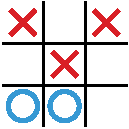
\includegraphics[width=0.15\textwidth]{figures/tic_ql_tab_move_1.pdf}
    } \hspace{0.1in}
    \subfloat[$Q(s_0, 2) = -1.0$]{
        \label{fig:tic-ql-tab-move-2}
        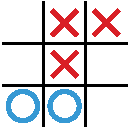
\includegraphics[width=0.15\textwidth]{figures/tic_ql_tab_move_2.pdf}
    } \hspace{0.1in}
    \subfloat[$Q(s_0, 4) = -1.0$]{
        \label{fig:tic-ql-tab-move-4}
        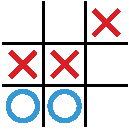
\includegraphics[width=0.15\textwidth]{figures/tic_ql_tab_move_4.pdf}
    } \hspace{0.1in}
    \subfloat[$Q(s_0, 6) = -1.0$]{
        \label{fig:tic-ql-tab-move-6}
        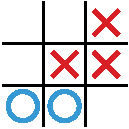
\includegraphics[width=0.15\textwidth]{figures/tic_ql_tab_move_6.pdf}
    } \hspace{0.1in}
    \subfloat[$Q(s_0, 9) = 1.0$]{
        \label{fig:tic-ql-tab-move-9}
        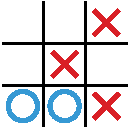
\includegraphics[width=0.15\textwidth]{figures/tic_ql_tab_move_9.pdf}
    }
    \caption{}
    \label{fig:tic-ql-qvalues}
\end{figure}

%%%%%%%%%%
% Figure %
%%%%%%%%%%

\begin{figure}[!h]
    \centering
    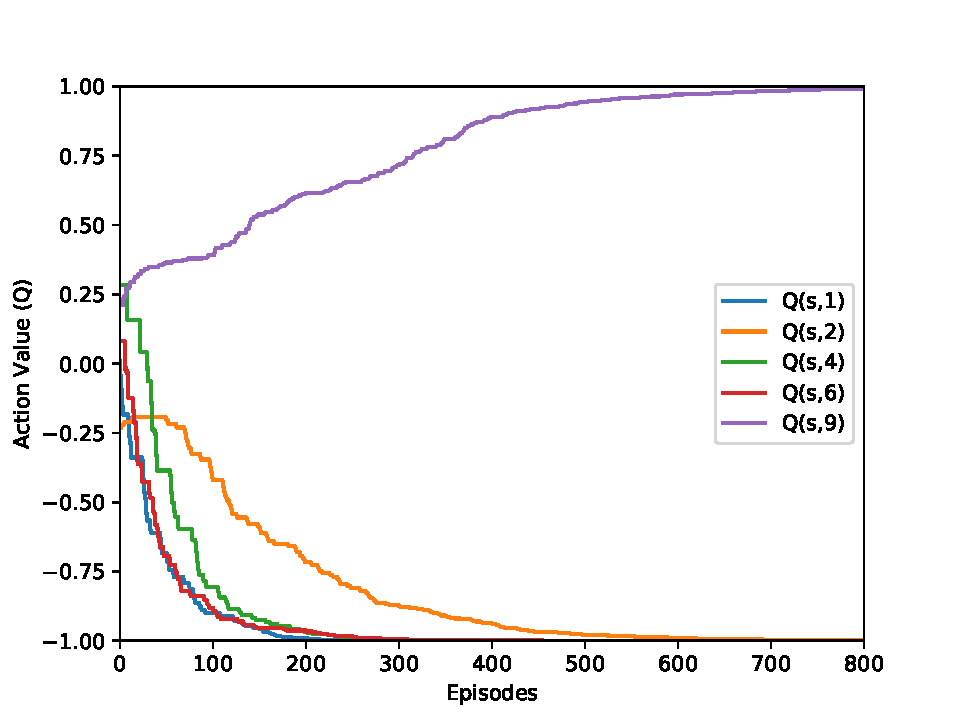
\includegraphics[width=0.40\textwidth]{figures/tic_ql_tab_action_values.pdf}
    \caption{The predicted state-action value during training.}
    \label{fig:tic-ql-tab-qvalues-progress}
\end{figure}

%%%%%%%%%%%%%%%%%%%%%%%%%
\subsubsection{Connect 4}
%%%%%%%%%%%%%%%%%%%%%%%%%

%%% MERGE THIS WITH PREVIOSU CHAPTER< SUBFIGURES

% \GithubURL{examples/c4_ql_tabular_fixed.py}{Implementation}

For Connect 4 we used the board position in \hyperref[fig:c4-ql-tab-cur]
{Figure~\ref*{fig:c4-ql-tab-cur}} as the starting state, $s_0$. It has three available actions,
$\mathcal{A}(s_0) = \{\texttt{d}, \texttt{f}, \texttt{g}\}$. By looking at such a simple position we
can clearly identify that the best available action is \texttt{f}, which leads to a win if we keep
playing the best possible actions.  Any other action (i.e. \texttt{d} or \texttt{g}) would lead to a
loss, assuming perfect play from the opponent.

%%%%%%%%%%
% Figure %
%%%%%%%%%%

\begin{figure}[!h]
    \centering
    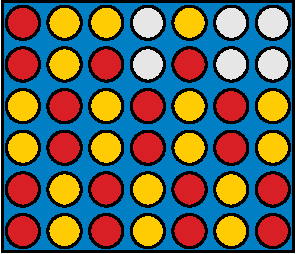
\includegraphics[width=0.2\textwidth]{figures/c4_ql_tab_current.pdf}
    \caption{Connect 4 board, $s_0$, with three legal actions: $\{\texttt{d}, \texttt{f}, \texttt{g}\}$.}
    \label{fig:c4-ql-tab-cur}
\end{figure}

We ran the same tabular version of the Q-learning algorithm with the same parameters as the used for
Tic-Tac-Toe $\alpha=0.1$ (learning rate), $\gamma=1.0$ (discount factor), and a uniformly random
behavior policy. The Q-values also converged to the expected values after around 800 episodes of
training, and are shown in \hyperref[fig:c4-ql-qvalues] {Figure~\ref*{fig:c4-ql-qvalues}}. As we can
see in \hyperref[fig:c4-ql-move-f] {Figure~\ref*{fig:c4-ql-move-f}}, the expected future reward of
taking action \texttt{f} is correctly estimated as 1.0, since that would lead to a win. At the same
time, the q-values for all the other actions was -1.0. This makes sense, since any action not being
\texttt{f} would lead to an immediate loss. Also, we can see in
\hyperref[fig:c4-ql-tab-qvalues-progress] {Figure~\ref*{fig:c4-ql-tab-qvalues-progress}} we can see
the predicted q-values for each available action. 

%%%%%%%%%%%
% Figures %
%%%%%%%%%%%

\begin{figure}[!h]
    \centering
    \subfloat[$Q(s_0, \texttt{d}) = -1.0$]{
        \label{fig:c4-ql-move-e}
        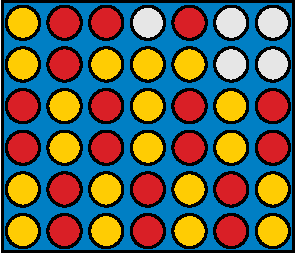
\includegraphics[width=0.2\textwidth]{figures/c4_ql_tab_move_d.pdf}
    } \hspace{0.1in}
    \subfloat[$Q(s_0, \texttt{f}) = 1.0$]{
        \label{fig:c4-ql-move-f}
        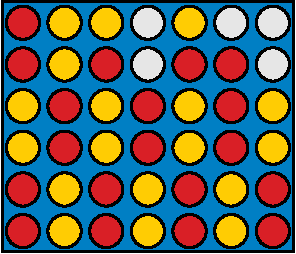
\includegraphics[width=0.2\textwidth]{figures/c4_ql_tab_move_f.pdf}
    } \hspace{0.1in}0
    \subfloat[$Q(s_0, \texttt{g}) = -1.0$]{
        \label{fig:c4-ql-move-g}
        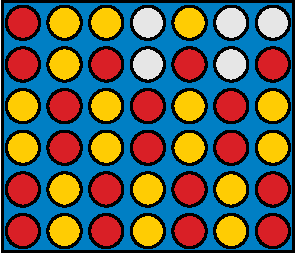
\includegraphics[width=0.2\textwidth]{figures/c4_ql_tab_move_g.pdf}
    }
    \caption{All the next states and their q values.}
    \label{fig:c4-ql-qvalues}
\end{figure}

%%%%%%%%%%
% Figure %
%%%%%%%%%%

\begin{figure}[!h]
    \centering
    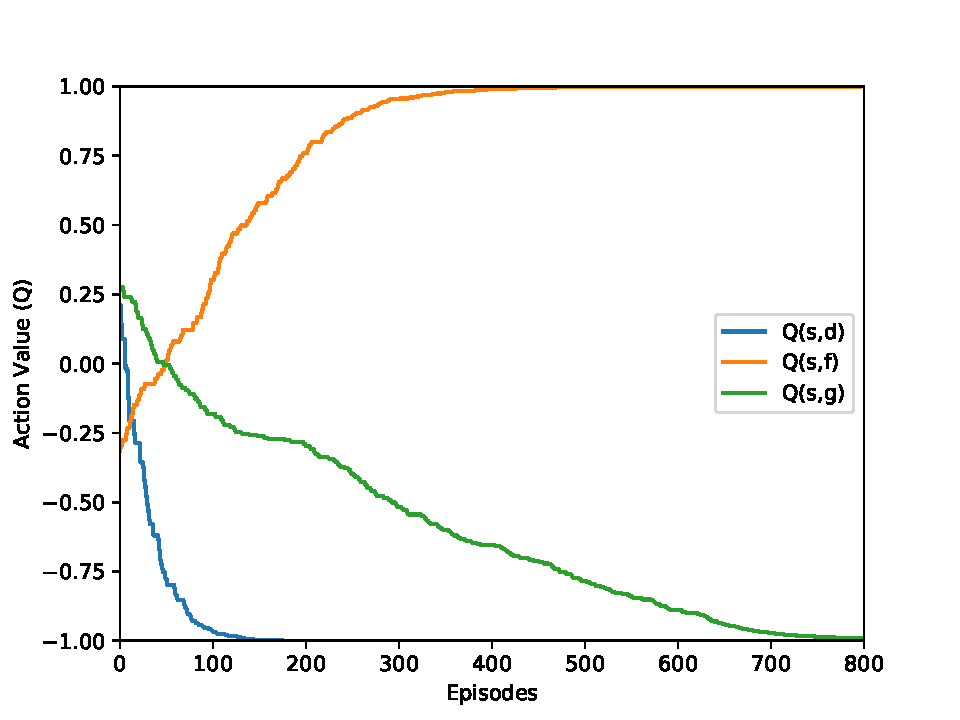
\includegraphics[width=0.50\textwidth]{figures/c4_ql_tab_action_values.pdf}
    \caption{The predicted state-action value during training.}
    \label{fig:c4-ql-tab-qvalues-progress}
\end{figure}

%%%%%%%%%%%%%%%%%%%%%%%%%%%%%%%%%%%%%%%%%%%%%%%%%%%%%%%%%%%%%
\subsection{Estimate q-values using Q-learning via self-play}
%%%%%%%%%%%%%%%%%%%%%%%%%%%%%%%%%%%%%%%%%%%%%%%%%%%%%%%%%%%%%

In the previous example we estimated the q-values for Tic-Tac-toe and Connect 4 positions against a
fixed Alpha-Beta opponent. While this works very well sometimes we don't have that algorithm. An
alternative is to use self-play, which consists in making playing games against itself.

% examples/tic_ql_tab_simple_selfplay.py 

%%%%%%%%%%%
% Figures %
%%%%%%%%%%%

\begin{figure}[!h]
    \centering
    \subfloat[Tic-Tac-Toe]{
        \label{fig:tic-ql-tab-simple-selfplay-progress}
        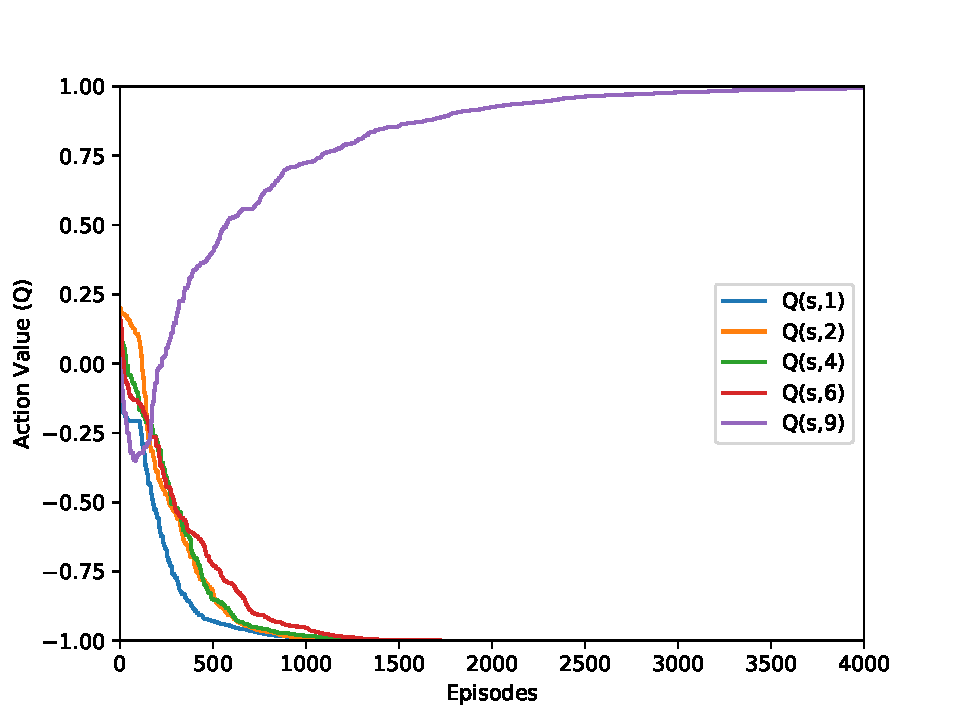
\includegraphics[width=0.4\textwidth]{figures/tic_ql_tab_simple_selfplay_progress.pdf}
    } \hspace{0.1in}
    \subfloat[Connect 4]{
        \label{fig:c4-ql-tab-simple-selfplay-progress}
        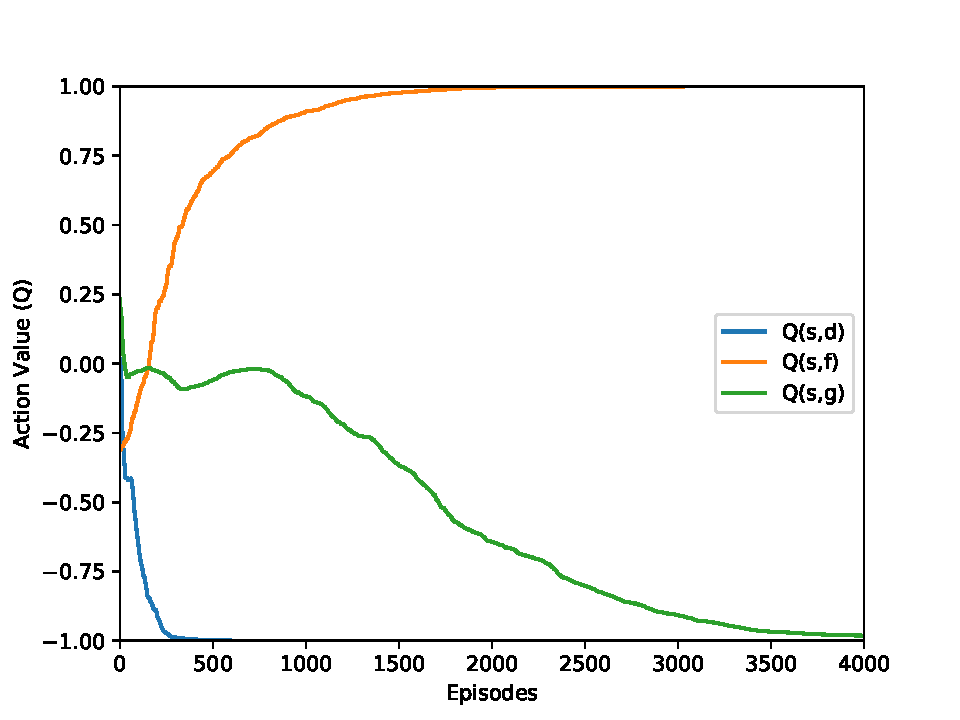
\includegraphics[width=0.4\textwidth]{figures/c4_ql_tab_simple_selfplay_progress.pdf}
    }
    \caption{All the next states and their q values.}
    \label{fig:ql-tab-simple-selfplay-progress}
\end{figure}

% This converged to examples/tic_ql_tab_simple_selfplay.py

In both examples we can see that it took longer to learn the episodes because it didn't have a
perfect guidance on what was good and bad, it had to learn it by itself. This is a powerful
technique that will be used in the next sections to learn a value function for Connect 4. The values
are the same as the ones shown in Figures \hyperref[fig:tic-ql-qvalues]{\ref*{fig:tic-ql-qvalues}}
and \hyperref[fig:c4-ql-qvalues]{\ref*{fig:c4-ql-qvalues}}.

%%%%%%%%%%%%%%%%%%%%%%%%%%%%%%%%%%%%%%%%%%%%%%%%%%%%%%%%%%%
\subsection{Estimate all q-values using tabular Q-learning}
%%%%%%%%%%%%%%%%%%%%%%%%%%%%%%%%%%%%%%%%%%%%%%%%%%%%%%%%%%%

% \GithubURL{examples/tic_ql_tab_full.py}{Implementation}

Now the idea is to learn to play the games in general starting from the same position. This means
that we will use Q-learning to estimate the q-values from the empty board of the game. We will do it
for Tic-Tac-Toe. We ran the experiment using similar parameters, and after 65,000 episodes the
q-values were found correctly.

% IDEA, Juntar ambos tic tac toe and connect 4 en uno!

In \hyperref[fig:tic-ql-tab-full-wld-plot]{Figure~\ref*{fig:tic-ql-tab-full-wld-plot}} we can see
how after 65,000 episodes it learned the values.

We were able to do that because the full game-tree of Tic-Tac-Toe is around 888888 game states. And
based on the results we can assume that the majority of the states were visited. But the problem now
is that Connect 4 has INSERT game states. That makes it impossible to run the Q-learning algorithm
with a tabular Q-function to save the exact value for every single state of the game. The solution
to this is now to use a function approximator.

\begin{figure}[!h]
    \centering
    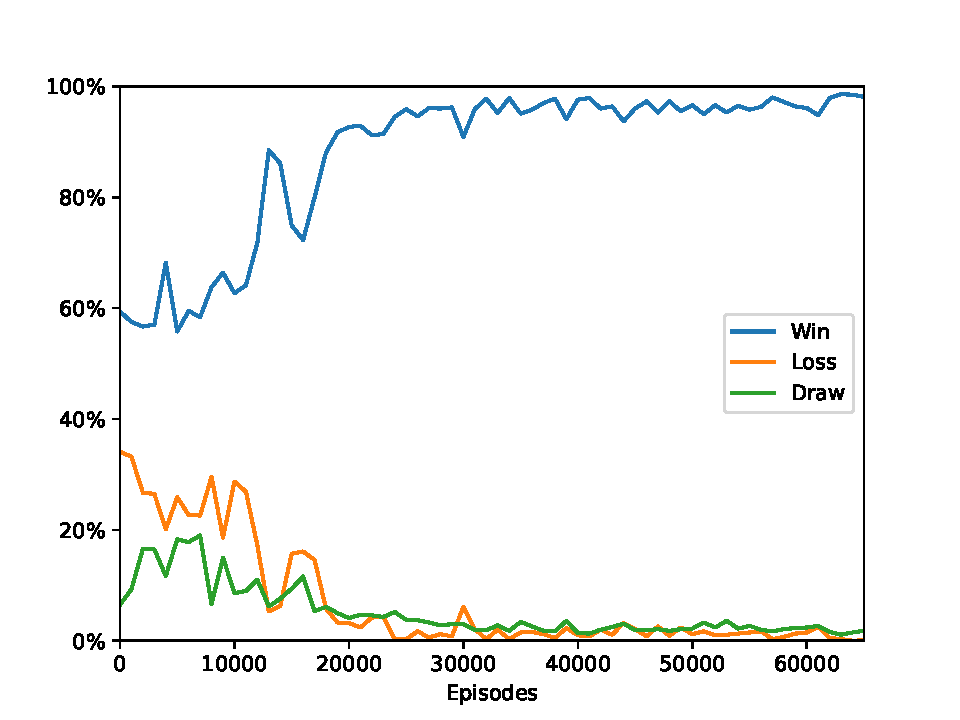
\includegraphics[width=0.50\textwidth]{figures/tic_ql_tab_full_wld_plot.pdf}
    \caption{Results after playing 1,000 games every 1,000 episodes against a Random player.}
    \label{fig:tic-ql-tab-full-wld-plot}
\end{figure}

sd fas dfas f sa fsad f asd fa s sd fas dfas f sa fsad f asd fa s sd fas dfas f sa fsad f asd fa s
sd fas dfas f sa fsad f asd fa s sd fas dfas f sa fsad f asd fa s sd fas dfas f sa fsad f asd fa s
sd fas dfas f sa fsad f asd fa s sd fas dfas f sa fsad f asd fa s sd fas dfas f sa fsad f asd fa s
sd fas dfas f sa fsad f asd fa s sd fas dfas f sa fsad f asd fa s sd fas dfas f sa fsad f asd fa s
sd fas dfas f sa fsad f asd fa s sd fas dfas f sa fsad f asd fa s sd fas dfas f sa fsad f asd fa s
sd fas dfas f sa fsad f asd fa s sd fas dfas f sa fsad f asd fa s sd fas dfas f sa fsad f asd fa s.

sd fas dfas f sa fsad f asd fa s sd fas dfas f sa fsad f asd fa s sd fas dfas f sa fsad f asd fa s
sd fas dfas f sa fsad f asd fa s sd fas dfas f sa fsad f asd fa s sd fas dfas f sa fsad f asd fa s
sd fas dfas f sa fsad f asd fa s sd fas dfas f sa fsad f asd fa s sd fas dfas f sa fsad f asd fa s
sd fas dfas f sa fsad f asd fa s sd fas dfas f sa fsad f asd fa s sd fas dfas f sa fsad f asd fa s
sd fas dfas f sa fsad f asd fa s sd fas dfas f sa fsad f asd fa s sd fas dfas f sa fsad f asd fa s
sd fas dfas f sa fsad f asd fa s sd fas dfas f sa fsad f asd fa s sd fas dfas f sa fsad f asd fa s.

%%%%%%%%%%%%%%%%%%%%%%%%%%%%%%%%%%%%%%%%%%%%%%%%%%%%%%%%%%%%%%%%%%%%%%%%%
\subsection{Estimate all q-values using tabular Q-learning via Self-Play}
%%%%%%%%%%%%%%%%%%%%%%%%%%%%%%%%%%%%%%%%%%%%%%%%%%%%%%%%%%%%%%%%%%%%%%%%%

% \GithubURL{examples/tic_ql_tab_full_selfplay.py}{Implementation}

\begin{figure}[!h]
    \centering
    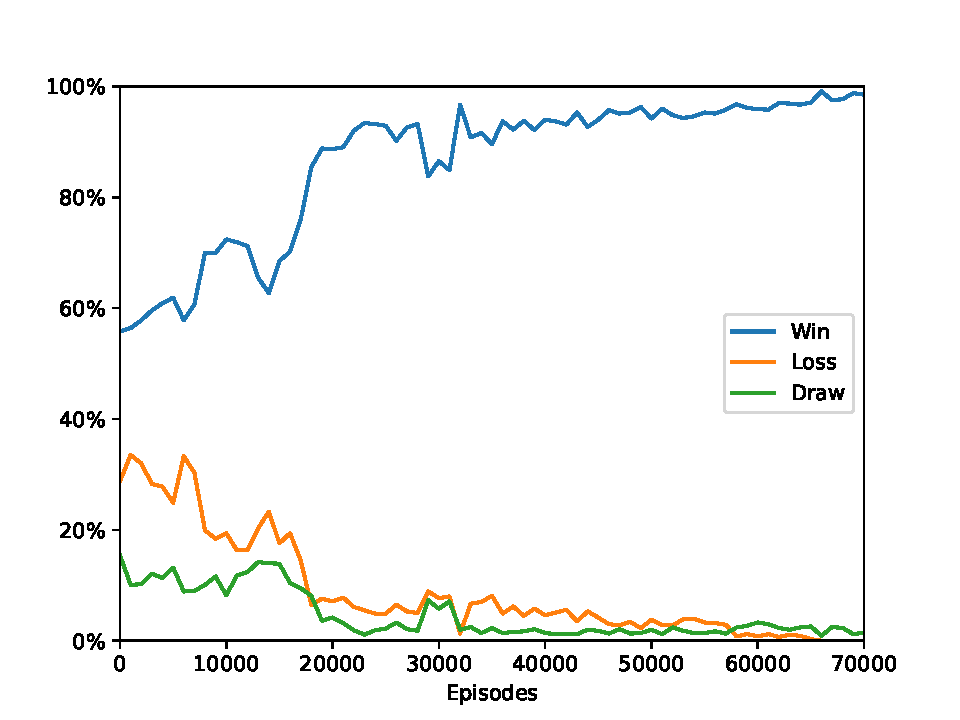
\includegraphics[width=0.50\textwidth]{figures/tic_ql_tab_full_selfplay_wld_plot.pdf}
    \caption{Results after playing 1,000 games every 1,000 episodes against a Random player.}
    \label{fig:tic-ql-tab-full-selfplay-wld-plot}
\end{figure}

In \hyperref[fig:tic-ql-tab-full-selfplay-wld-plot]
{Figure~\ref*{fig:tic-ql-tab-full-selfplay-wld-plot}} we can see how after 70,000 episodes it
learned the values.

sd fas dfas f sa fsad f asd fa s sd fas dfas f sa fsad f asd fa s sd fas dfas f sa fsad f asd fa s
sd fas dfas f sa fsad f asd fa s sd fas dfas f sa fsad f asd fa s sd fas dfas f sa fsad f asd fa s
sd fas dfas f sa fsad f asd fa s sd fas dfas f sa fsad f asd fa s sd fas dfas f sa fsad f asd fa s
sd fas dfas f sa fsad f asd fa s sd fas dfas f sa fsad f asd fa s sd fas dfas f sa fsad f asd fa s
sd fas dfas f sa fsad f asd fa s sd fas dfas f sa fsad f asd fa s sd fas dfas f sa fsad f asd fa s
sd fas dfas f sa fsad f asd fa s sd fas dfas f sa fsad f asd fa s sd fas dfas f sa fsad f asd fa s.

sd fas dfas f sa fsad f asd fa s sd fas dfas f sa fsad f asd fa s sd fas dfas f sa fsad f asd fa s
sd fas dfas f sa fsad f asd fa s sd fas dfas f sa fsad f asd fa s sd fas dfas f sa fsad f asd fa s
sd fas dfas f sa fsad f asd fa s sd fas dfas f sa fsad f asd fa s sd fas dfas f sa fsad f asd fa s
sd fas dfas f sa fsad f asd fa s sd fas dfas f sa fsad f asd fa s sd fas dfas f sa fsad f asd fa s
sd fas dfas f sa fsad f asd fa s sd fas dfas f sa fsad f asd fa s sd fas dfas f sa fsad f asd fa s
sd fas dfas f sa fsad f asd fa s sd fas dfas f sa fsad f asd fa s sd fas dfas f sa fsad f asd fa s.

%%%%%%%%%%%%%%%%%%%%%%%%%%%%%%%%%%%%%%%%%%%%%%%%%%%%%%%%%%%
\subsection{Estimate Q-values Using Approximate Q-learning}
%%%%%%%%%%%%%%%%%%%%%%%%%%%%%%%%%%%%%%%%%%%%%%%%%%%%%%%%%%%

sd fas dfas f sa fsad f asd fa s sd fas dfas f sa fsad f asd fa s sd fas dfas f sa fsad f asd fa s
sd fas dfas f sa fsad f asd fa s sd fas dfas f sa fsad f asd fa s sd fas dfas f sa fsad f asd fa s
sd fas dfas f sa fsad f asd fa s sd fas dfas f sa fsad f asd fa s sd fas dfas f sa fsad f asd fa s
sd fas dfas f sa fsad f asd fa s sd fas dfas f sa fsad f asd fa s sd fas dfas f sa fsad f asd fa s
sd fas dfas f sa fsad f asd fa s sd fas dfas f sa fsad f asd fa s sd fas dfas f sa fsad f asd fa s
sd fas dfas f sa fsad f asd fa s sd fas dfas f sa fsad f asd fa s sd fas dfas f sa fsad f asd fa s.

sd fas dfas f sa fsad f asd fa s sd fas dfas f sa fsad f asd fa s sd fas dfas f sa fsad f asd fa s
sd fas dfas f sa fsad f asd fa s sd fas dfas f sa fsad f asd fa s sd fas dfas f sa fsad f asd fa s
sd fas dfas f sa fsad f asd fa s sd fas dfas f sa fsad f asd fa s sd fas dfas f sa fsad f asd fa s
sd fas dfas f sa fsad f asd fa s sd fas dfas f sa fsad f asd fa s sd fas dfas f sa fsad f asd fa s
sd fas dfas f sa fsad f asd fa s sd fas dfas f sa fsad f asd fa s sd fas dfas f sa fsad f asd fa s
sd fas dfas f sa fsad f asd fa s sd fas dfas f sa fsad f asd fa s sd fas dfas f sa fsad f asd fa s.

%%%%%%%%%%%%%%%%%%%%%%%%%%%%%%%%%%%%%%%%%%%%%%%%%%%%%%%%%%%%%%%%%%%%%%%%%%%%%%%%%%%%%%%%%%%%%%%%%%%%
\section{Results}
%%%%%%%%%%%%%%%%%%%%%%%%%%%%%%%%%%%%%%%%%%%%%%%%%%%%%%%%%%%%%%%%%%%%%%%%%%%%%%%%%%%%%%%%%%%%%%%%%%%%

%%%%%%%%%%%%%%%%%%%%%%%%%%%%%%%%%%%%%%%%%%%%
\subsection{Model Evaluation and Validation}
%%%%%%%%%%%%%%%%%%%%%%%%%%%%%%%%%%%%%%%%%%%%

Content.

%%%%%%%%%%%%%%%%%%%%%%%%%%
\subsection{Justification}
%%%%%%%%%%%%%%%%%%%%%%%%%%

Content.

%%%%%%%%%%%%%%%%%%%%%%%%%%%%%%%%%%%%%%%%%%%%%%%%%%%%%%%%%%%%%%%%%%%%%%%%%%%%%%%%%%%%%%%%%%%%%%%%%%%%
\section{Conclusion}
%%%%%%%%%%%%%%%%%%%%%%%%%%%%%%%%%%%%%%%%%%%%%%%%%%%%%%%%%%%%%%%%%%%%%%%%%%%%%%%%%%%%%%%%%%%%%%%%%%%%

%%%%%%%%%%%%%%%%%%%%%%%%%%%%%%%%%%%%
\subsection{Free-Form Visualization}
%%%%%%%%%%%%%%%%%%%%%%%%%%%%%%%%%%%%

Content.

%%%%%%%%%%%%%%%%%%%%%%%
\subsection{Reflection}
%%%%%%%%%%%%%%%%%%%%%%%

Content.

%%%%%%%%%%%%%%%%%%%%%%%%
\subsection{Improvement}
%%%%%%%%%%%%%%%%%%%%%%%%

Content.

%%%%%%%%%%%%%%%%%%%%%%%%%%%%%%%%%%%%%%%%%%%%%%%%%%%%%%%%%%%%%%%%%%%%%%%%%%%%%%%%%%%%%%%%%%%%%%%%%%%%
% BIBLIOGRAPHY
%%%%%%%%%%%%%%%%%%%%%%%%%%%%%%%%%%%%%%%%%%%%%%%%%%%%%%%%%%%%%%%%%%%%%%%%%%%%%%%%%%%%%%%%%%%%%%%%%%%%

\bibliographystyle{plainnat}
\bibliography{bibliography}

\end{document}
